\documentclass[table,dvipsnames,10pt]{beamer}
\mode<presentation>{
	\usetheme{Madrid}
	\setbeamercolor{title}{fg=Black,bg=Blue!15}
	\setbeamercolor{frametitle}{fg=Black,bg=Blue!15}
	\setbeamercolor{block title}{fg=Black,bg=Blue!15}
	\setbeamercolor{block}{fg=Black,bg=Blue!10}
}

\usepackage{default}
\usepackage{graphicx}
\usepackage{booktabs}
\usepackage{xcolor}
\usepackage{multirow}
\usepackage{minted}
\usepackage[
type={CC},
modifier={by-sa},
version={4.0},
]{doclicense}

\definecolor{LightGray}{gray}{0.9}

\title[Audiometri Development]{Laporan Uji Audiometri}
\author{}
\institute[VibrasticLab : \ccbysa]{
	Achmadi ST MT\\
	\medskip
	\textit{}
}
\date{}

\begin{document}
	\section{Start}
	
	\begin{frame}
	\titlepage
	\end{frame}

	\begin{frame}
	\frametitle{Requirement}
	
	\begin{exampleblock}{General}
		Membangun unit produk audiometri untuk penggunaan medis 
	\end{exampleblock}

	\begin{exampleblock}{User Requirement}
	\begin{itemize}
		\item \textbf{Portabel}. 
		\begin{itemize}
			\item \textbf{Self Power source}. Dapat berupa battery sekali pakai maupun \textit{rechargeable}.
			
			\item \textbf{Ukuran}. Unit harus memiliki ukuran volume kecil dan massa yang ringan.
						
			\item \textbf{Interface}. Unit harus menggunakan \textit{interface} atau antar muka yang terintegrasi dengan unit produk.
			
		\end{itemize}
		
		\item \textbf{Storage}. Unit harus memiliki metode atau part untuk menyimpan hasil pengukuran.
		
		\item \textbf{Intuitif}. Unit harus mengikuti standar produk intuitif sehingga pengguna
		dapat mengoperasikan unit dengan sedikit atau tanpa sama sekali membutuhkan panduan.
	\end{itemize}
	\end{exampleblock}
	\end{frame}

	\begin{frame}
	\frametitle{Requirement}
	\begin{exampleblock}{Technical Requirement}
		\begin{itemize}
			\item Unit harus menggunakan daya VDD (3.3 volt) atau VCC (5 volt) dengan konsumsi arus rendah.
			
			\item Unit harus menggunakan komponen seminimal mungkin agar ukurannya kecil dan ringan.
			
			\item Unit harus dilengkapi \textit{interface} atau antar-muka pengguna.
			Lebih detil:
			\begin{itemize}
				\item Untuk input cukuplah tombol-tombol push button.
				\item Untuk display cukuplah LCD atau LED indikator.
				\item Jika memungkinkan, jadikan satu input dan display
				dalam bentuk layar sentuh LCD-TFT.
			\end{itemize}
			\item Unit harus memiliki emulasi \textit{filesystem} untuk media peyimpanan seperti
			SDCard, MMC, atau USB-Flashdisk.
			
			\item Unit harus menyembunyikan semua kompleksitas teknis sehingga mudah digunakan pengguna.
			Jika membutuhkan perangkat lain maka wajib perangkat tersebut sudah lazim tersedia.
		\end{itemize}
	\end{exampleblock}
	\end{frame}

	\begin{frame}
	\frametitle{Requirement}
	\begin{exampleblock}{Measurement Goals}
		\begin{enumerate}
			\item Apakah tone yang dihasilkan hanya satu frekuensi dan bersih dari frekuensi derau?
			\item Bagaimana pergeseran frekuensi terhadap perubahan clock maupun panjang array buffer?
			\item Bagaimana pergeseran amplitudo terhadap maximum SPL di frekuensi yang diinginkan?
			\item Bagaimana hubungan pergeseran frekuensi terhadap amplitudo frekuensi yang diinginkan?
			\item Apakah array buffer yang dihasilkan sudah sesuai dengan array untuk channel mono?
			\item Apakah masih menghasilkan \textit{audio-pop} saat menghasilkan tone?
		\end{enumerate}
	\end{exampleblock}
	\end{frame}

	\begin{frame}
	\frametitle{Design}
	\begin{exampleblock}{Simplified Schematic}
		\begin{figure}[H]
			\centering
			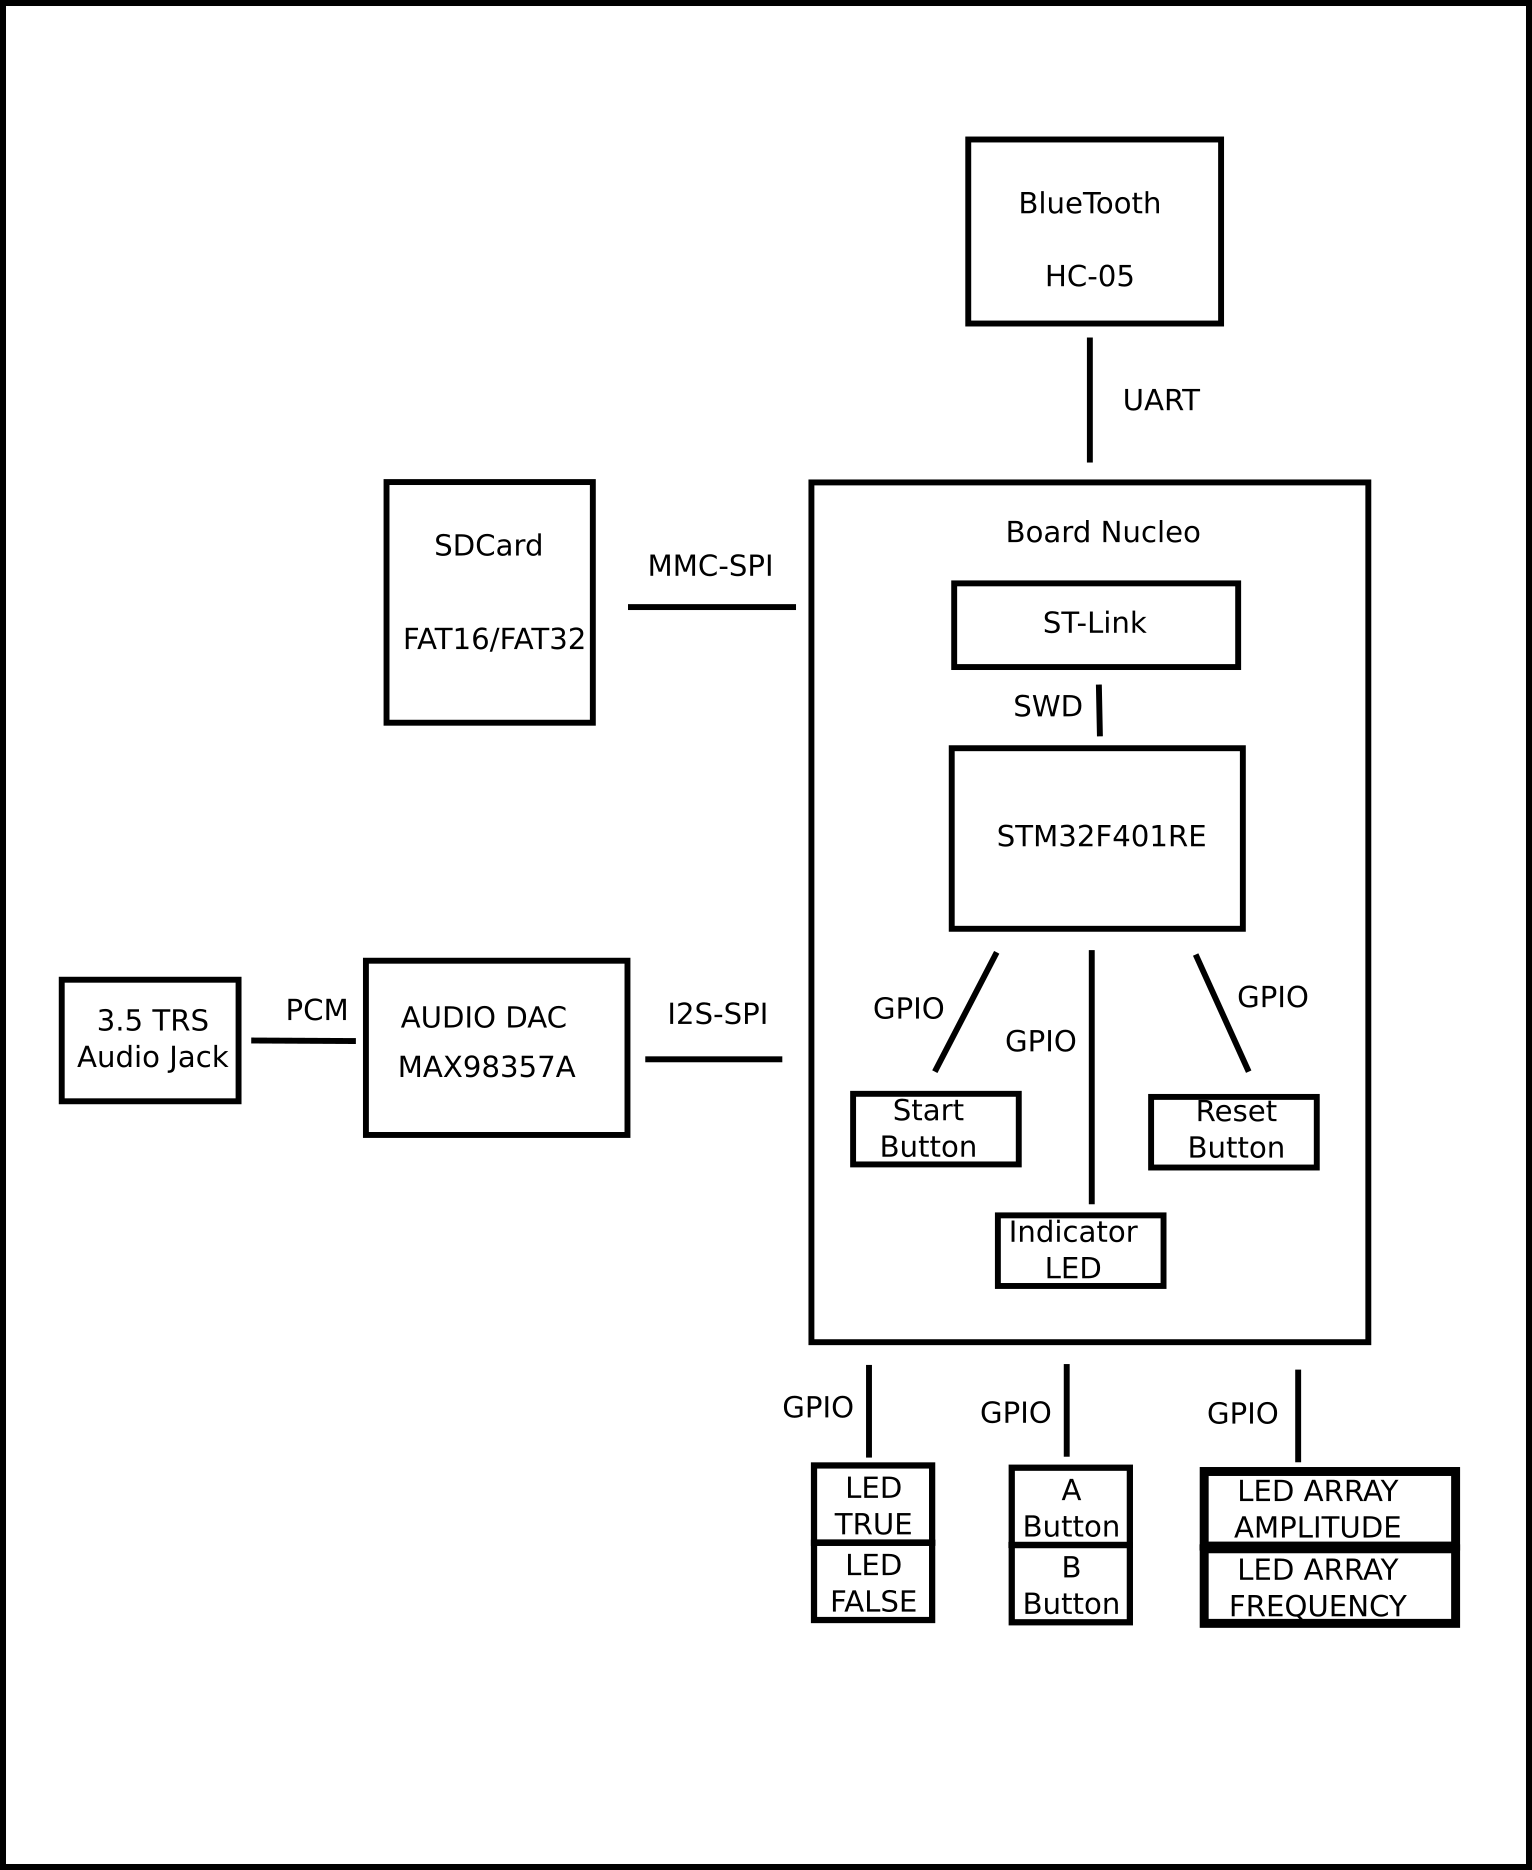
\includegraphics[width=0.55\linewidth]{images/overview}
		\end{figure}
	\end{exampleblock}	
	\end{frame}

	\begin{frame}
	\frametitle{Design}
	\begin{exampleblock}{CPU chip varian}
		Menggunakan chip microcontroller STMF4 atau yang satu family.
	\end{exampleblock}
	\begin{exampleblock}{Why STM32?}
		\begin{itemize}
			\item ARM 32-bit Cortex-M4.
			\item Tegangan daya 3.3V.
			\item Ukuran kecil standar paket TQFP.
			\item Tersedia protokol FSMC untuk layar-sentuh LCD-TFT.
			\item Tersedia protokol SPI-FatFs untuk media SDCard/MMC.
			\item Tersedia protokol SPI-I2S untuk Audio PCM.
			\item Tersedia total 144 pin GPIO untuk LED dan tombol.
			\item Harga sangat terjangkau untuk fitur yang tersedia.
		\end{itemize}
	\end{exampleblock}	
	\end{frame}
	
	
	\begin{frame}
	\frametitle{Design}
	\begin{exampleblock}{Audio DAC}
		Menggunakan chip Audio DAC (Digital to Analog Converter) MAX98357A
	\end{exampleblock}
	\begin{exampleblock}{Why MAX98357A}
		\begin{itemize}
			\item Class-D Amplifier.
			\item Tegangan daya 3.3V atau 5V tanpa butuh tegangan negatif.
			\item Protokol PCM 16-bit standar I2S (Inter-Integrated Sound).
			\item Output langsung ke coil/speaker tanpa tambahan amplifier lain.
			\item Tersedia pilihan gain 3dB, 6dB, 9dB (default), 12dB, dan 15dB.
			\item Tersedia fitur Shut-Down untuk \textit{High-Impedance}
			saat tidak menghasilkan output apapun.
		\end{itemize}
	\end{exampleblock}	
	\end{frame}

	\begin{frame}
	\frametitle{Sinyal}
	\begin{exampleblock}{PCM 16-bit}
		PCM (\textit{Pulse-Coded Modulation}) adalah protokol standar untuk bertukar data audio digital.
		Setiap satu frame data PCM terdiri dari 32 bit data untuk channel kanan dan kiri masing-masing 16-bit.
		Jumlah frame mengikuti panjang array buffer yang digunakan.
	\end{exampleblock}
	\begin{exampleblock}{Diagram sinyal}
			\begin{figure}[H]
			\centering
			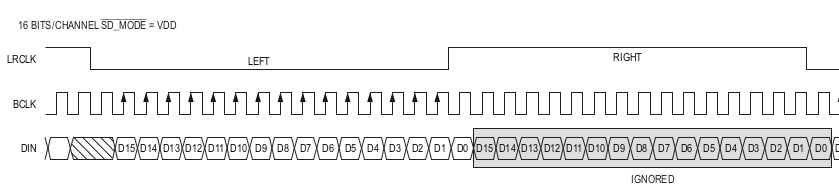
\includegraphics[width=\linewidth]{images/PCM}
		\end{figure}
	\end{exampleblock}	
	\end{frame}

	\begin{frame}
	\frametitle{Sinyal}
	\begin{exampleblock}{Sinyal Name}
	\begin{itemize}
		\item \textbf{LRCLK (Left/Right Clock)}. Sinyal untuk kontrol bagian kanan dan kiri.
		Mengingat chip MAX98357A adalah \textit{mono-amplifier},
		maka posisi sinyal kanan (atau LRCLK berlogika \textit{high}) akan diabaikan.
		
		\item \textbf{BCLK (Bit Clock)}. Sinyal clock untuk kirim data.
		Chip MAX98357A akan membaca nilai bit data di setiap tepi-naik (\textit{Rising-Edge})
		dari sinyal BCLK.
		
		\item \textbf{DIN (Data IN)}. Sinyal bit data.
		Satu frame 32-bit Left/Right berasal dari satu variabel elemen dari array buffer.
	\end{itemize}
	\end{exampleblock}
	\begin{exampleblock}{}
			Di chip STM32, modulasi PCM dikirim melalui protokol I2S (\textit{Inter-Integrated Sound})
			via jalur SPI (\textit{Serial Peripheral Interface}).
	\end{exampleblock}
	\begin{exampleblock}{}		
			Secara berurutan, koneksi untuk SPI (MOSI-SCK-NSS) dan untuk I2S (DIN-BCLK-LRCLK).
	\end{exampleblock}	
	\end{frame}

	\begin{frame}
	\frametitle{Amplifier}
	\begin{exampleblock}{Class-D} 
		Class-D adalah jenis amplifier yang tidak mengambil sinyal analog sebagai input.
		Sebaliknya menggunakan sinyal digital PWM (Pulse-Width Modulation) atau PCM (Pulse-Coded Modulation) sebagai input.
	\end{exampleblock}
	\begin{exampleblock}{}
		Sinyal input ini kemudian ditumpangkan (dimodulasi) ke PWM frekuensi tinggi dan diamplifikasi sesuai nilai gain.
		Kemudian dengan \textit{low-pass filter}, sinyal dikonversi menjadi lebih analog
		dengan membuang PWM frekuensi tinggi yang "tersisa" di output.
	\end{exampleblock}
	\begin{exampleblock}{}
		Chip MAX98357A menggunakan sinyal dasar \textit{squared} PWM pada frekuensi 300kHz.
		Untuk low-pass filter, digunakan Capasitor 220pF dan Ferrit/Inductor.
	\end{exampleblock}
	\end{frame}

	\begin{frame}
	\frametitle{Amplifier}
	\begin{exampleblock}{Schematic} 
		\begin{figure}[H]
			\centering
			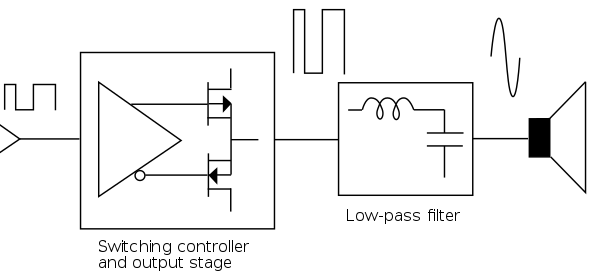
\includegraphics[width=0.6\linewidth]{images/classD}
		\end{figure}
	\end{exampleblock}
	\begin{exampleblock}{} 
		\begin{figure}[H]
			\centering
			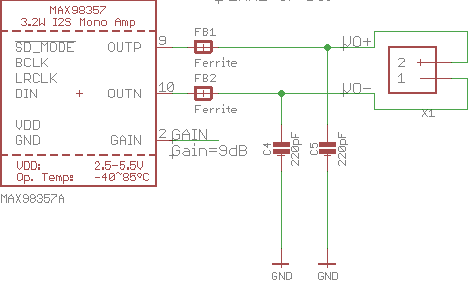
\includegraphics[width=0.45\linewidth]{images/max98357A}
		\end{figure}
	\end{exampleblock}
	\end{frame}

	\begin{frame}
	\frametitle{Essential Programming}
	\begin{exampleblock}{Important files} 
		Seluruh \textit{source-code} tersedia di repository github milik Lab Vibrastik.
		Beberapa file penting untuk dievaluasi terkait tone generator:
		
		\begin{itemize}
			\item \textbf{mcuconf.h}. Berisi pengaturan clock untuk STM32 dan fitur I2S.\\
			\url{https://github.com/VibrasticLab/pikoakustik/blob/master/nucleo401/mcuconf.h}
			
			\item \textbf{ht\_audio.h}. Berisi makro/definisi untuk fitur tone generator.\\
			\url{https://github.com/VibrasticLab/pikoakustik/blob/master/nucleo401/ht_audio.h}
			
			\item \textbf{ht\_audio.c}. Berisi referensi dan implementasi proses tone generator.\\
			\url{https://github.com/VibrasticLab/pikoakustik/blob/master/nucleo401/ht_audio.c}
		\end{itemize}
	\end{exampleblock}
	\end{frame}

	\begin{frame}[fragile]
	\frametitle{Essential Programming}
	\begin{exampleblock}{Clock Setting} 
		Pengaturan clock untuk peripheral SPI-I2S pada default 96 MHz.
		\begin{minted}[frame=lines,framesep=2mm,fontsize=\tiny,bgcolor=LightGray]{c}
#define STM32_PLLM_VALUE    16
#define STM32_PLLN_VALUE    384
#define STM32_PLLP_VALUE    8
#define STM32_I2SSRC        STM32_I2SSRC_PLLI2S
#define STM32_PLLI2SN_VALUE 288
#define STM32_PLLI2SR_VALUE 3
		\end{minted}
	\end{exampleblock}

	\begin{exampleblock}{Variabel array buffer} 
		Ukuran variabel adalah 16-bit (sesuai ukuran bit PCM).
		Panjang array total harus cukup panjang untuk menghindari
		noise akibat zero-padding yang tidak tercapai.
		\begin{minted}[frame=lines,framesep=2mm,fontsize=\tiny,bgcolor=LightGray]{c}
uint16_t i2s_tx_buf[512*16];
		\end{minted}
	\end{exampleblock}
	\end{frame}

	\begin{frame}[fragile]
	\frametitle{Essential Programming}
	\begin{exampleblock}{I2S Driver configuration} 
		Disini dimasukkan variabel array buffer.
		Juga didefinisikan ukuran buffer yang akan di \textit{play-loop}.
		Ukuran buffer play ini harus lebih kecil daripada total array buffer
		dan akan mempengaruhi frekuensi tone yang dihasilkan.
		Ukuran buffer play default adalah 512.
		Frekuensi BCLK diatur pada 16kHz.
		\begin{minted}[frame=lines,fontsize=\footnotesize]{c}
I2SConfig i2scfg = {
	i2s_tx_buf,
	NULL,
	512,
	NULL,
	0,
	16,
};
		\end{minted}
	\end{exampleblock}
	\end{frame}

	\begin{frame}[fragile]
	\frametitle{Essential Programming}
	\begin{exampleblock}{Zero Array} 
\[ Y(i) = 0, \text{ for } 0 \leq i < 512 \]
	\end{exampleblock}
	\begin{exampleblock}{} 
	\begin{minted}[frame=lines,fontsize=\footnotesize]{c}
for(i=0;i<512;i++){
	i2s_tx_buf[i] = 0;
}
	\end{minted}
	\end{exampleblock}

	\begin{exampleblock}{Sine Array} 
		\[ Y(i) = sin(2\pi f \frac{i}{512}), \text{ for } 0 \leq i < 512 \]
	\end{exampleblock}
	\begin{exampleblock}{} 
		\begin{minted}[frame=lines,fontsize=\footnotesize]{c}
for(i=0;i<512;i++){
	i2s_tx_buf[i] = sin(freq*i*2*(M_PI/512));
}
		\end{minted}
	\end{exampleblock}
	\end{frame}

	\begin{frame}
	\frametitle{Preparing}
	\begin{exampleblock}{Skema}
		\begin{figure}[H]
			\centering
			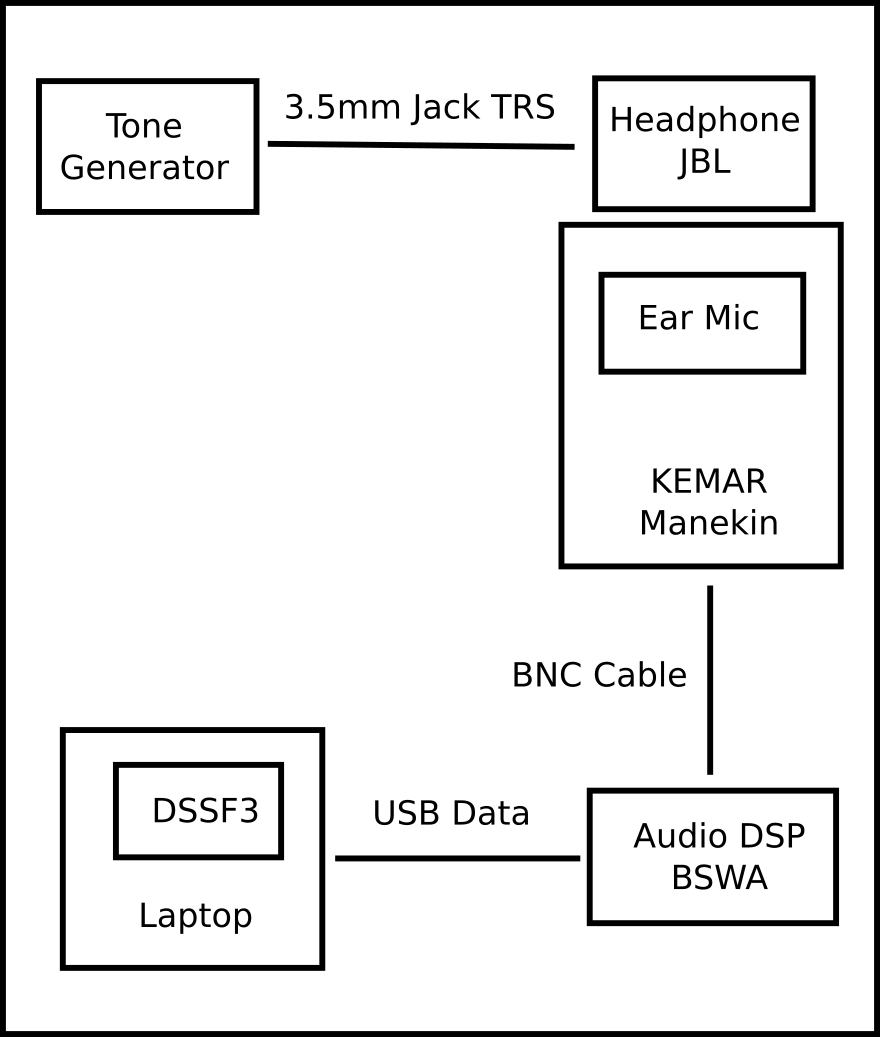
\includegraphics[width=0.5\linewidth]{images/kemar}
		\end{figure} 
	\end{exampleblock}
	\end{frame}

	\begin{frame}
	\frametitle{Preparing}
	\begin{exampleblock}{Manekin dan Earleaf}
		\begin{figure}[H]
			\centering
			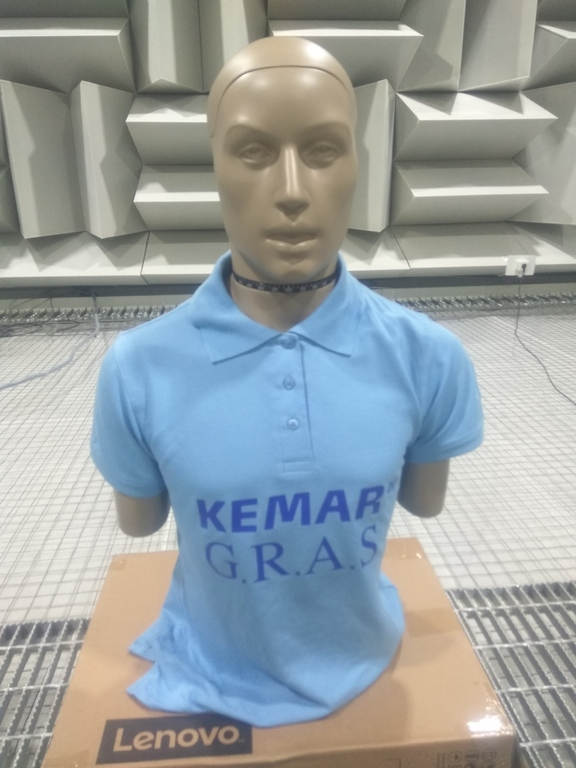
\includegraphics[width=0.3\linewidth]{day_1/manekin0}
			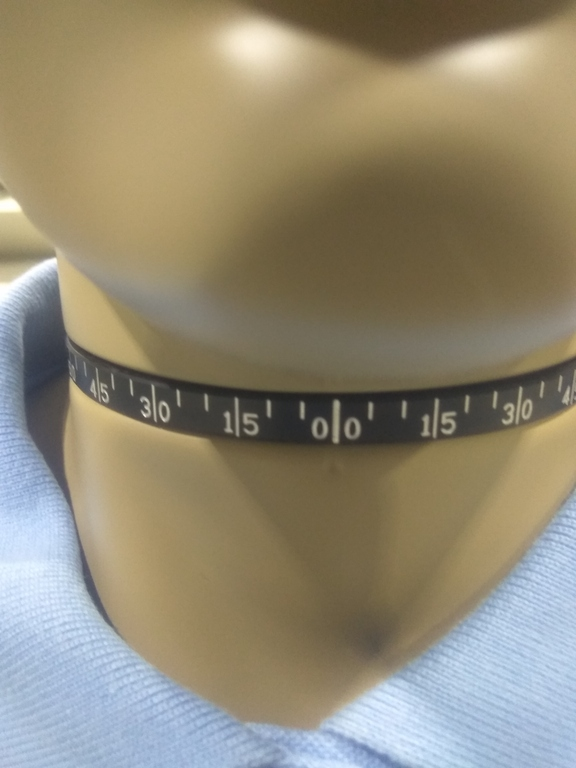
\includegraphics[width=0.3\linewidth]{day_1/manekin1}
			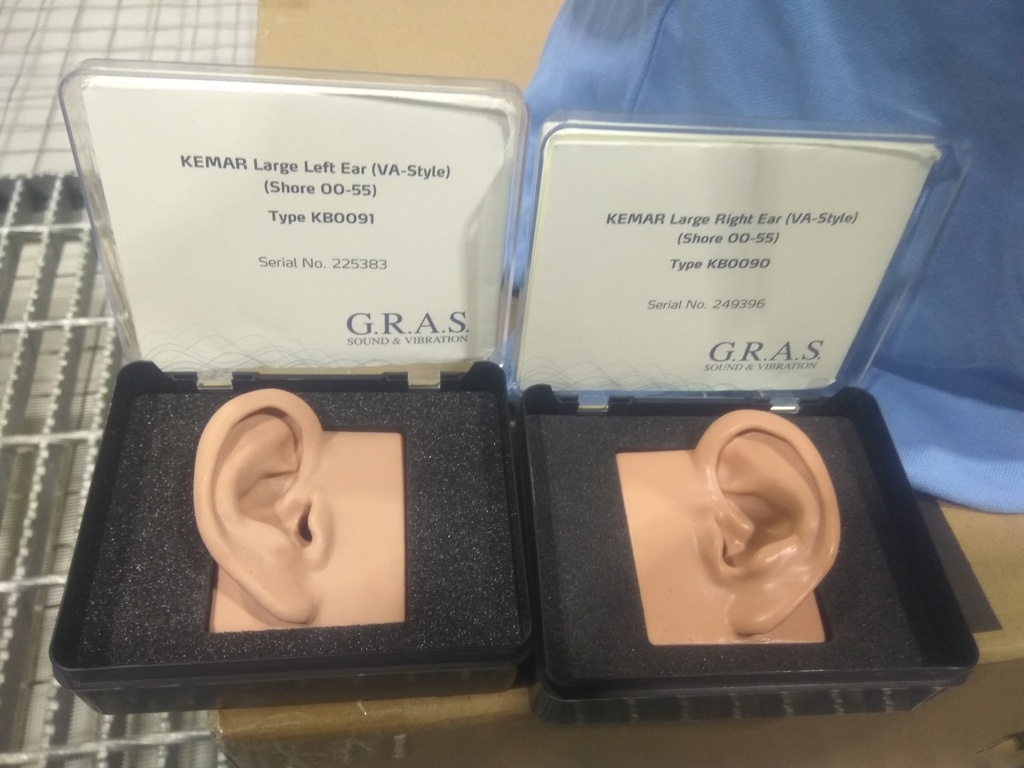
\includegraphics[width=0.3\linewidth]{day_1/earleaf0}
		\end{figure}
	\end{exampleblock}
	\end{frame}

	\begin{frame}
	\frametitle{Preparing}
	\begin{exampleblock}{Wiring BNC cable}
		\begin{figure}[H]
			\centering
			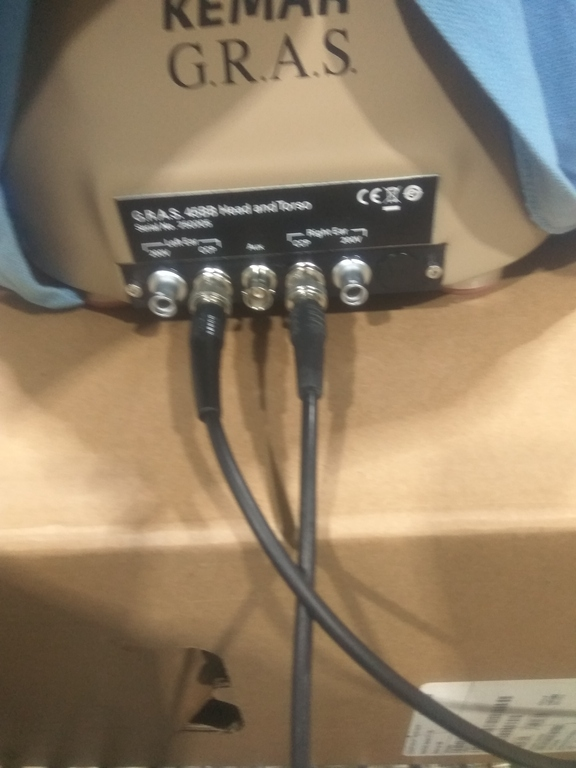
\includegraphics[width=0.3\linewidth]{day_1/wiring0}
			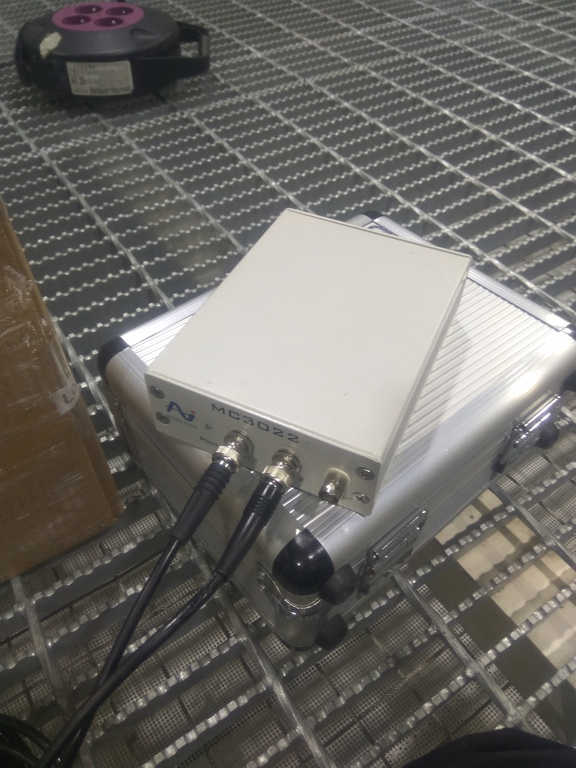
\includegraphics[width=0.3\linewidth]{day_1/wiring1}
		\end{figure}
	\end{exampleblock}
	\end{frame}

	\begin{frame}
	\frametitle{Preparing}
	\begin{exampleblock}{Kalibrasi}
		Acuan standar kalibrasi pada SPL 114 dB dan frekuensi 250 Hz
		\begin{figure}[H]
			\centering
			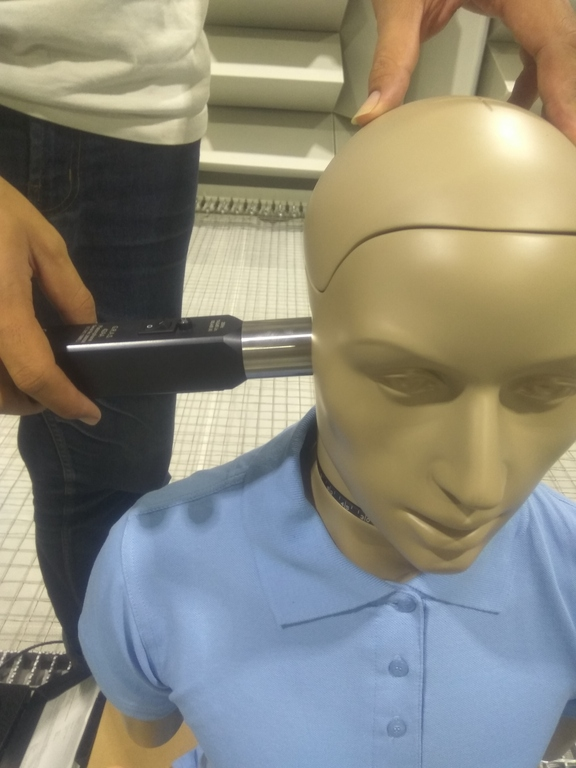
\includegraphics[width=0.3\linewidth]{day_1/kalib0}
			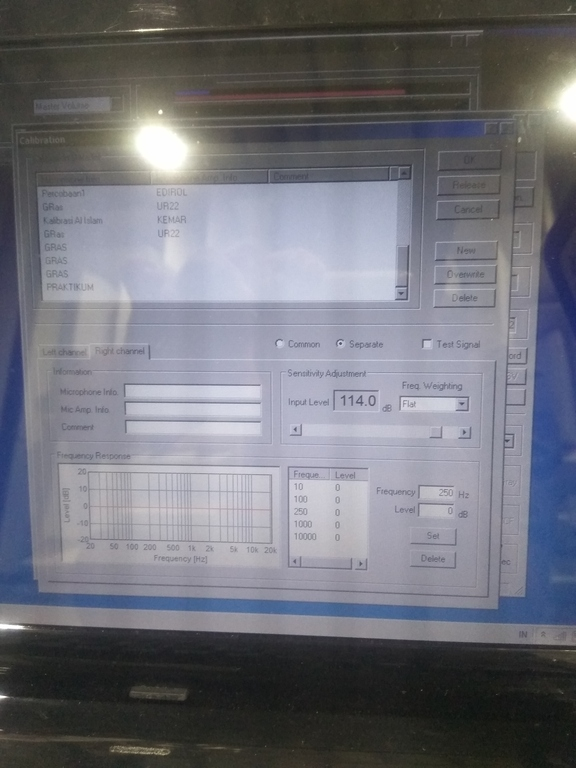
\includegraphics[width=0.3\linewidth]{day_1/kalib1}
			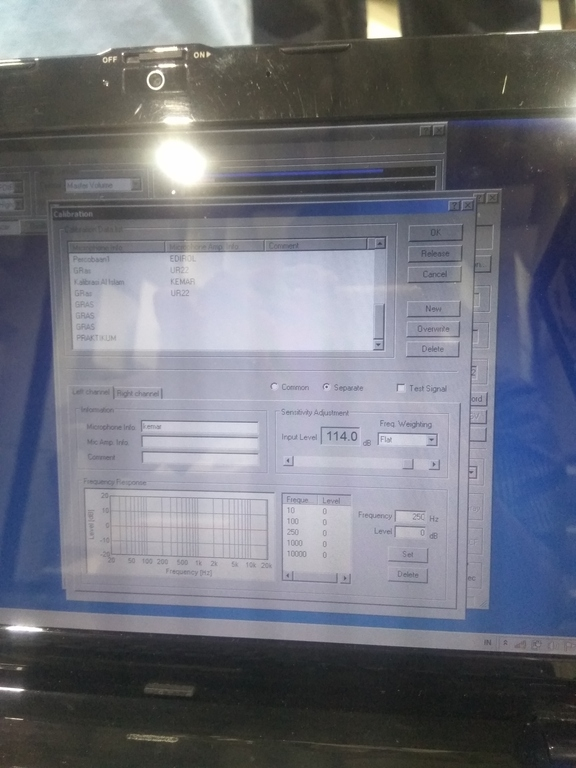
\includegraphics[width=0.3\linewidth]{day_1/kalib2}
		\end{figure}
	\end{exampleblock}
	\end{frame}

	\begin{frame}
	\frametitle{Preparing}
	\begin{exampleblock}{Earleaf}
		\begin{figure}[H]
			\centering
			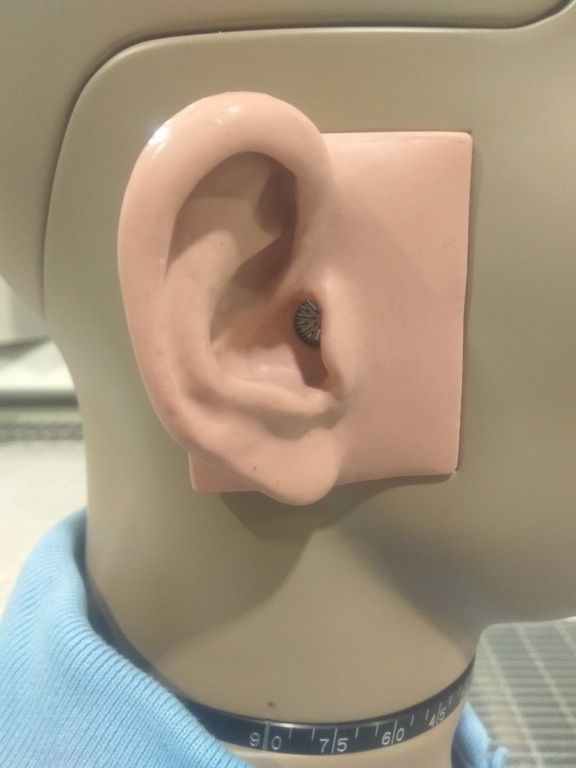
\includegraphics[width=0.15\linewidth]{day_1/earleaf1}
			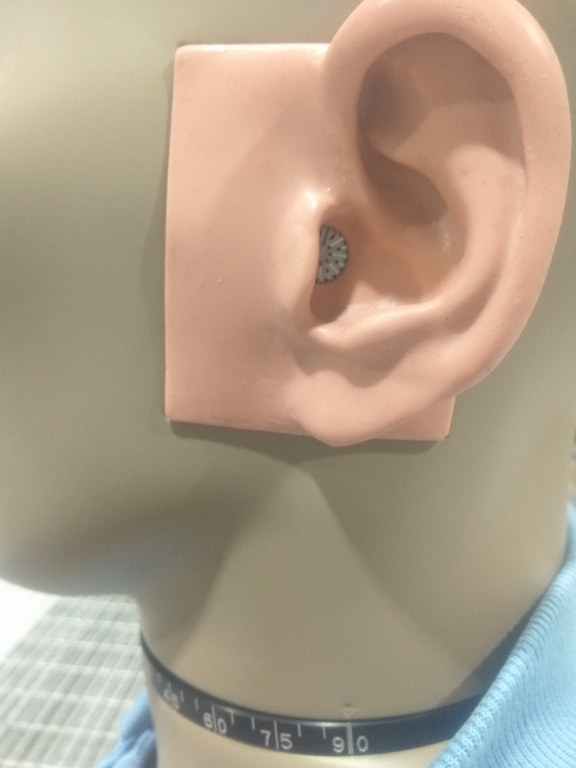
\includegraphics[width=0.15\linewidth]{day_1/earleaf2}
		\end{figure}
	\end{exampleblock}

	\begin{exampleblock}{Headphone}
		\begin{figure}[H]
			\centering
			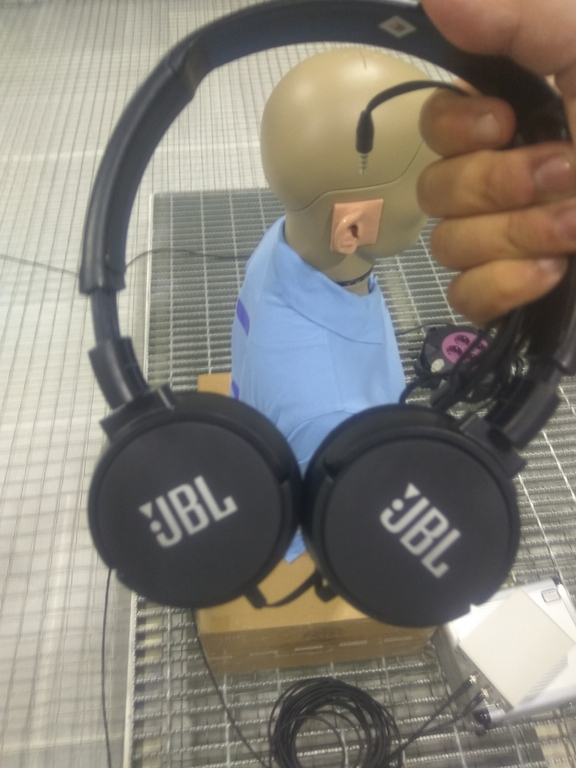
\includegraphics[width=0.15\linewidth]{day_1/phone0}
			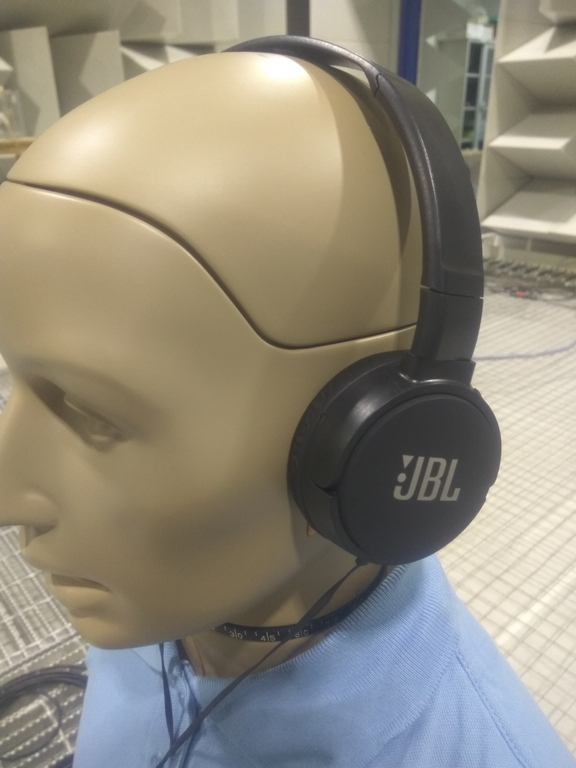
\includegraphics[width=0.15\linewidth]{day_1/phone1}
			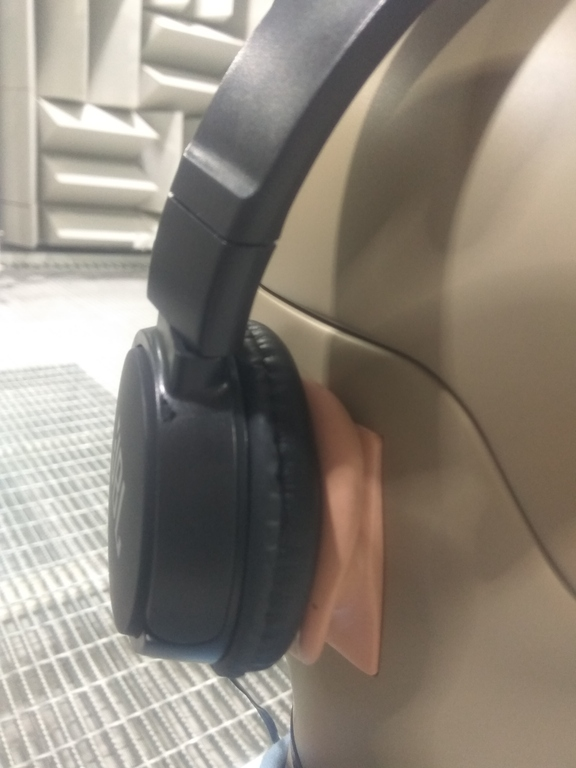
\includegraphics[width=0.15\linewidth]{day_1/phone2}
		\end{figure}
	\end{exampleblock}
	\end{frame}

	\begin{frame}
	\frametitle{Preparing}
	\begin{exampleblock}{First Test}
		\begin{figure}[H]
			\centering
			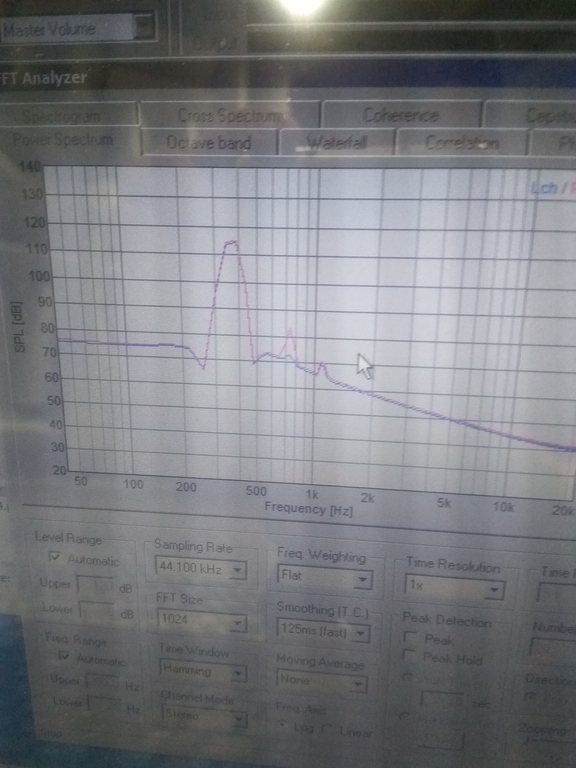
\includegraphics[width=0.3\linewidth]{day_1/test0}
			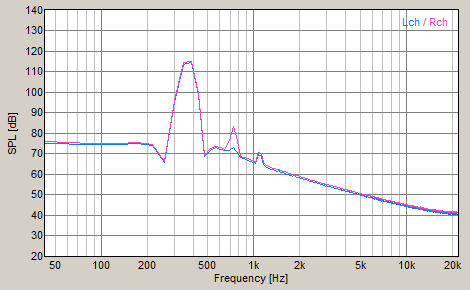
\includegraphics[width=0.6\linewidth]{day_1/test1}
		\end{figure}
	\end{exampleblock}
	\end{frame}

	\begin{frame}
	\frametitle{Test Sine Array}
	\begin{exampleblock}{Table reversed-sine}
		\begin{figure}[H]
			\centering
			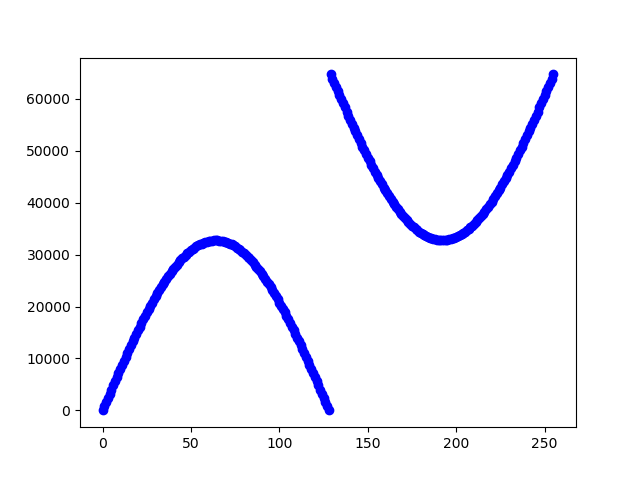
\includegraphics[width=0.45\linewidth]{result/day_1/rev_sine_table}
			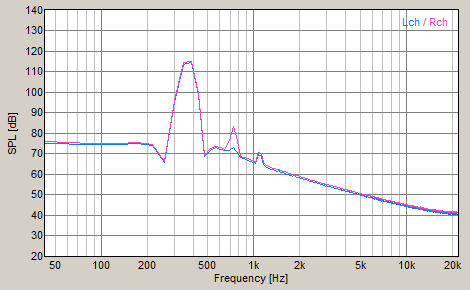
\includegraphics[width=0.45\linewidth]{result/day_1/tableMax256}
		\end{figure}
	\end{exampleblock}
	\end{frame}

	\begin{frame}[fragile]
	\frametitle{Test Sine Array}
	\begin{exampleblock}{Formula reversed-sine}
		\[
		Y(i) =
		\begin{cases}
		A sin(\pi \frac{i}{127}), \text{ if } 0 \leq i < 127\\
		A(2-sin(\pi \frac{i}{127})), \text{ if } 127 \leq i < 256\\
		\end{cases}
		\]
	\end{exampleblock}
	\begin{exampleblock}{}
		\begin{minted}[frame=lines,fontsize=\footnotesize]{c}
for(i=0;i<127;i++){
	i2s_tx_buf[i]=32767*sin(3.141592653589793*(i/127));
	i2s_tx_buf[127+i]=32767*(2-sin(3.141592653589793*(i/127)));
}
		\end{minted}
	\end{exampleblock}
	\begin{exampleblock}{}
		\begin{figure}[H]
			\centering
			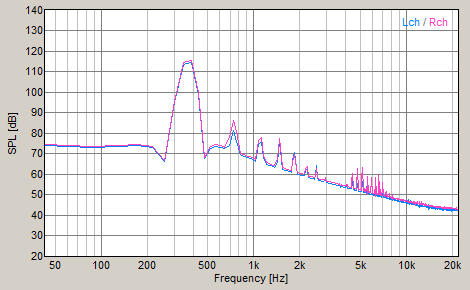
\includegraphics[width=0.45\linewidth]{result/day_1/halfMax256}
		\end{figure}
	\end{exampleblock}
	\end{frame}

	\begin{frame}[fragile]
	\frametitle{Test Sine Array}
	\begin{exampleblock}{Formula sine}
		\[ Y(i) = A sin(2\pi f \frac{i}{256}), \text{ for } 0 \leq i < 256 \]
	\end{exampleblock}
	\begin{exampleblock}{}
		\begin{minted}[frame=lines,fontsize=\footnotesize]{c}
for(i=0;i<256;i++){
	i2s_tx_buf[i] = 32767*sin( i*2*(M_PI/256));
}
		\end{minted}
	\end{exampleblock}
	\begin{exampleblock}{}
		\begin{figure}[H]
			\centering
			\includegraphics[width=0.45\linewidth]{result/day_1/Max256}
		\end{figure}
	\end{exampleblock}
	\end{frame}

	\begin{frame}[fragile]
	\frametitle{Test Sine Variasi panjang Array}
	\begin{exampleblock}{512}
		\begin{figure}[H]
			\centering
			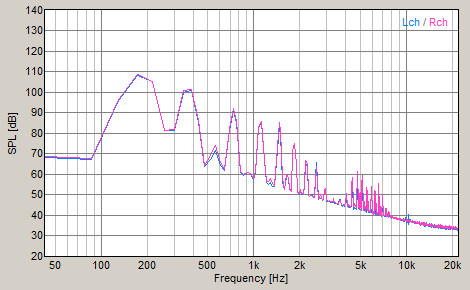
\includegraphics[width=0.4\linewidth]{result/day_1/max512}
		\end{figure}
	\end{exampleblock}
	\begin{exampleblock}{1024}
		\begin{figure}[H]
			\centering
			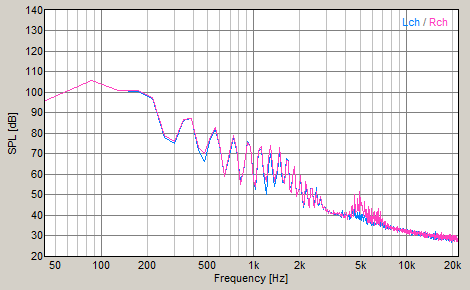
\includegraphics[width=0.4\linewidth]{result/day_1/max1024}
		\end{figure}
	\end{exampleblock}
	\end{frame}

	\begin{frame}[fragile]
	\frametitle{Test Sine Variasi Clock I2S}
	\begin{exampleblock}{Clock 48MHz}
		\begin{minted}[frame=lines,fontsize=\footnotesize]{c}
#define STM32_PLLI2SN_VALUE 288
#define STM32_PLLI2SR_VALUE 6
		\end{minted}
	\end{exampleblock}
	\begin{exampleblock}{}
		\begin{figure}[H]
		\centering
		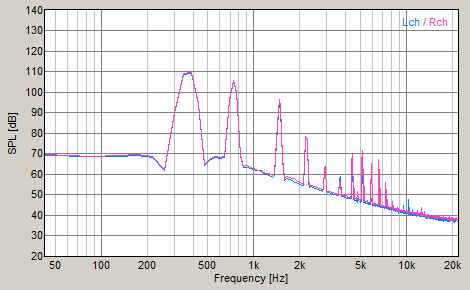
\includegraphics[width=0.5\linewidth]{result/day_2/sine_clk48}
	\end{figure}
	\end{exampleblock}
	\end{frame}

	\begin{frame}[fragile]
	\frametitle{Test Sine Variasi Clock I2S}
	\begin{exampleblock}{Clock 72MHz}
		\begin{minted}[frame=lines,fontsize=\footnotesize]{c}
#define STM32_PLLI2SN_VALUE 288
#define STM32_PLLI2SR_VALUE 4
		\end{minted}
	\end{exampleblock}
	\begin{exampleblock}{}
		\begin{figure}[H]
			\centering
			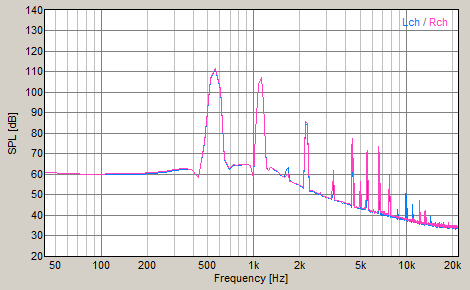
\includegraphics[width=0.5\linewidth]{result/day_2/sine_clk72}
		\end{figure}
	\end{exampleblock}
	\end{frame}

	\begin{frame}[fragile]
	\frametitle{Test Sine Variasi Clock I2S}
	\begin{exampleblock}{Clock 96MHz}
		\begin{minted}[frame=lines,fontsize=\footnotesize]{c}
#define STM32_PLLI2SN_VALUE 288
#define STM32_PLLI2SR_VALUE 3
		\end{minted}
	\end{exampleblock}
	\begin{exampleblock}{}
		\begin{figure}[H]
			\centering
			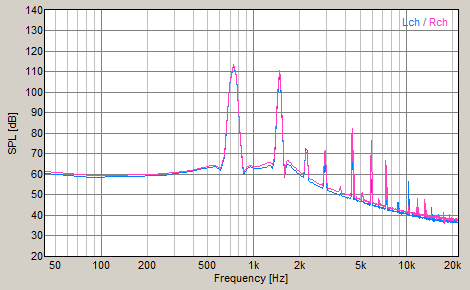
\includegraphics[width=0.5\linewidth]{result/day_2/sine_clk96}
		\end{figure}
	\end{exampleblock}
	\end{frame}

	\begin{frame}[fragile]
	\frametitle{Test Sine Overflow signed 16-bit}
	\begin{exampleblock}{}
		\[
		Y(i) =
		\begin{cases}
		A sin(2 \pi \frac{i}{512}), \text{ if } Y \geq 0, \text{ for } 0 \leq i < 512\\
		A sin(2 \pi \frac{i}{512})+65535, \text{ if } Y < 0, \text{ for } 0 \leq i < 512
		\end{cases}
		\]
	\end{exampleblock}
	\begin{exampleblock}{}
		\begin{minted}[frame=lines,fontsize=\footnotesize]{c}
for(i=0;i<512;i++){
	ysin = 32767*sin(2*3.141592653589793*(i/512));
	if(ysin >= 0){ i2s_tx_buf[i]=ysin; }
	if(ysin <0  ){ i2s_tx_buf[i]=ysin+65535; }
}
		\end{minted}
	\end{exampleblock}
	\begin{exampleblock}{}
		\begin{figure}[H]
			\centering
			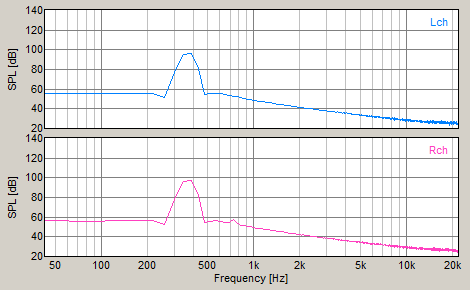
\includegraphics[width=0.45\linewidth]{result/day_4/newsine400fft}
			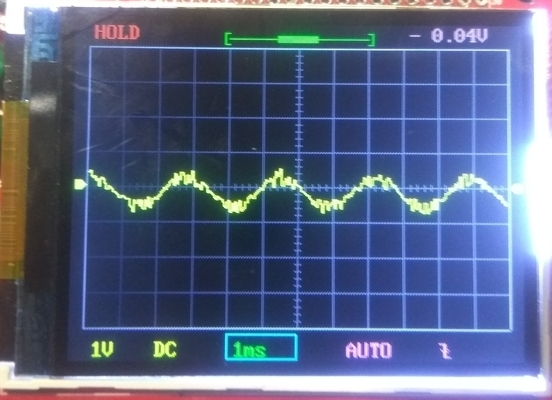
\includegraphics[width=0.4\linewidth]{result/day_4/goodsine2}
		\end{figure}
	\end{exampleblock}
	\end{frame}

	\begin{frame}[fragile]
	\frametitle{Test modifikasi panjang array}
	\begin{exampleblock}{}
		\[ B = 512/F \]
		\[
		Y(i) =
		\begin{cases}
		A sin(2 \pi \frac{i}{B}), \text{ if } Y \geq 0, \text{ for } 0 \leq i < B\\
		A sin(2 \pi \frac{i}{B})+65535, \text{ if } Y < 0, \text{ for } 0 \leq i < B
		\end{cases}
		\]
	\end{exampleblock}
	\begin{exampleblock}{}
\begin{minted}[frame=lines,fontsize=\footnotesize]{c}
buffsize = (uint16_t) 512/freq;
for(i=0;i<buffsize;i++){
	ysin = 32767*sin(2*3.141592653589793*(i/buffsize));
	if(ysin >= 0){ i2s_tx_buf[i]=ysin; }
	if(ysin <0  ){ i2s_tx_buf[i]=ysin+65535; }
}
i2scfg.size = buffsize;
		\end{minted}
	\end{exampleblock}
	\begin{exampleblock}{Nilai Amplitudo dan Frekuensi }
		\[ f = \frac{f_{left} + f_{right}}{2} \text{ , } P = \frac{P_{left} + P_{right}}{2}\]
	\end{exampleblock}
	\end{frame}

	\begin{frame}[fragile]
	\frametitle{Test modifikasi panjang array}
	\begin{exampleblock}{Skala Frekuensi 1 atau panjang array 512}
		Aktual $freq = 387$ Hz dan $SPL = 97 dB$
		\begin{figure}[H]
			\centering
			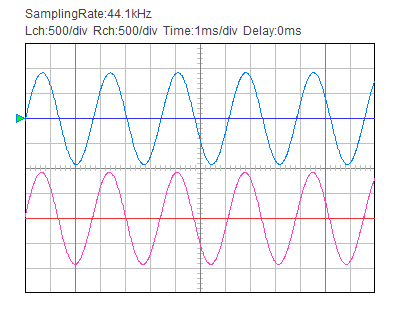
\includegraphics[width=0.4\linewidth]{result/day_4/newsine400}
			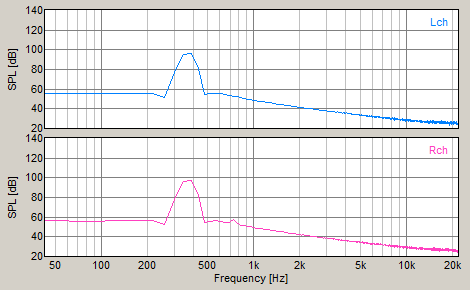
\includegraphics[width=0.45\linewidth]{result/day_4/newsine400fft}
		\end{figure}
	\end{exampleblock}
	\end{frame}

	\begin{frame}[fragile]
	\frametitle{Test modifikasi panjang array}
	\begin{exampleblock}{Skala Frekuensi 2 atau panjang array 256}
		Aktual $freq = 732 Hz$ dan $SPL = 101 dB$
		\begin{figure}[H]
			\centering
			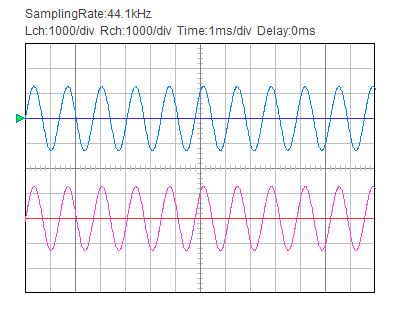
\includegraphics[width=0.4\linewidth]{result/day_4/osi_sine2}
			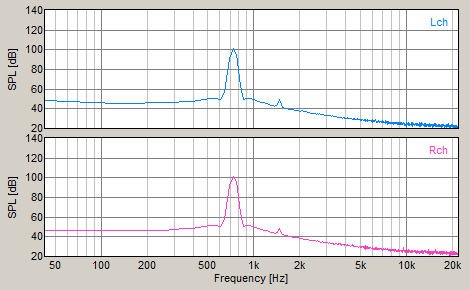
\includegraphics[width=0.45\linewidth]{result/day_4/fft_sine2}
		\end{figure}
	\end{exampleblock}
	\end{frame}

	\begin{frame}[fragile]
	\frametitle{Test modifikasi panjang array}
	\begin{exampleblock}{Skala Frekuensi 4 atau panjang array 128}
		Aktual $freq = 1464 Hz$ dan $SPL = 110 dB$
		\begin{figure}[H]
			\centering
			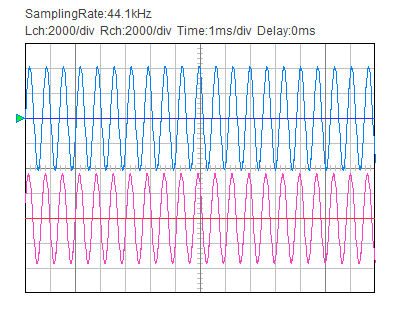
\includegraphics[width=0.4\linewidth]{result/day_4/osi_sine4}
			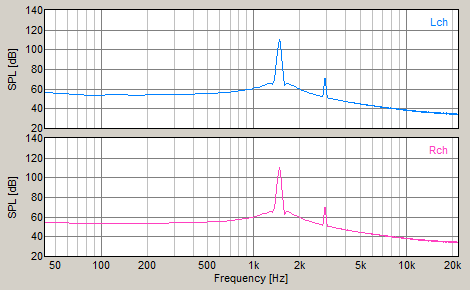
\includegraphics[width=0.45\linewidth]{result/day_4/fft_sine4}
		\end{figure}
	\end{exampleblock}
	\end{frame}

	\begin{frame}[fragile]
	\frametitle{Test modifikasi panjang array}
	\begin{exampleblock}{Skala Frekuensi 8 atau panjang array 64}
		Aktual $freq = 2971 Hz$ dan $SPL = 91 dB$
		\begin{figure}[H]
			\centering
			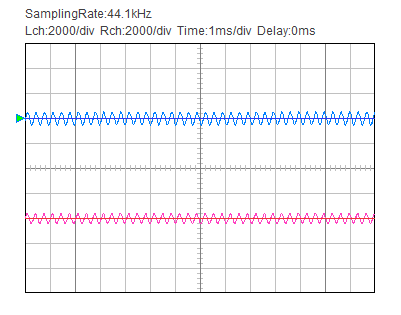
\includegraphics[width=0.4\linewidth]{result/day_4/osi_sine8}
			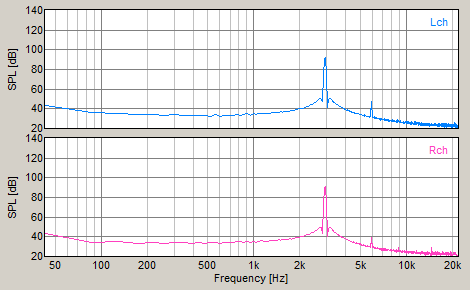
\includegraphics[width=0.45\linewidth]{result/day_4/fft_sine8}
		\end{figure}
	\end{exampleblock}
	\end{frame}

	\begin{frame}[fragile]
	\frametitle{Test modifikasi panjang array}
	\begin{exampleblock}{Skala Frekuensi 16 atau panjang array 32}
		Aktual $freq = 5900 Hz$ dan $SPL = 90 dB$
		\begin{figure}[H]
			\centering
			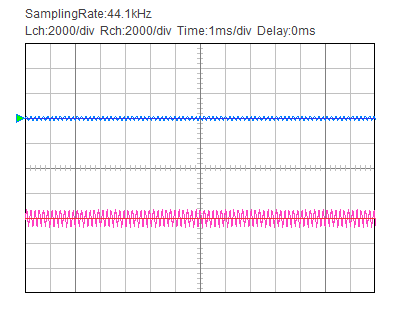
\includegraphics[width=0.4\linewidth]{result/day_4/osi_sine16}
			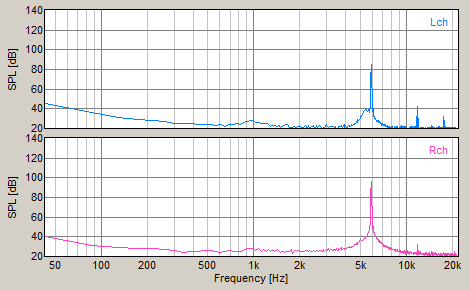
\includegraphics[width=0.45\linewidth]{result/day_4/fft_sine16}
		\end{figure}
	\end{exampleblock}
	\end{frame}

	\begin{frame}[fragile]
	\frametitle{Test modifikasi panjang array}
	\begin{exampleblock}{Skala Frekuensi 32 atau panjang array 16}
		Aktual $freq = 11800 Hz$ dan $SPL = 85 dB$
		\begin{figure}[H]
			\centering
			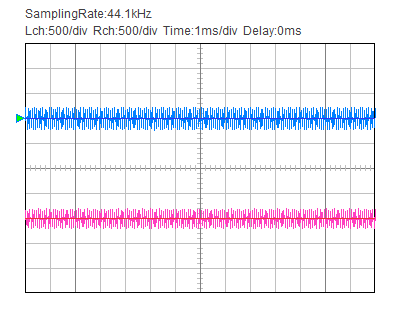
\includegraphics[width=0.4\linewidth]{result/day_4/newsinehighest}
			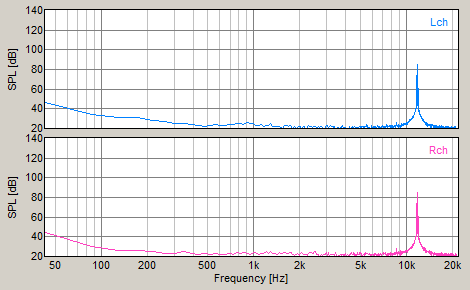
\includegraphics[width=0.45\linewidth]{result/day_4/newsinehighestfft}
		\end{figure}
	\end{exampleblock}
	\end{frame}

	\begin{frame}[fragile]
	\frametitle{Test modifikasi panjang array}
	\begin{exampleblock}{Skala Frekuensi 0.5 atau panjang array 1024}
		Aktual $freq = 172 Hz$ dan $SPL = 96 dB$
		\begin{figure}[H]
			\centering
			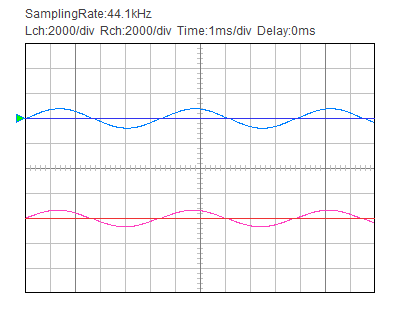
\includegraphics[width=0.4\linewidth]{result/day_4/osi_sine0p5}
			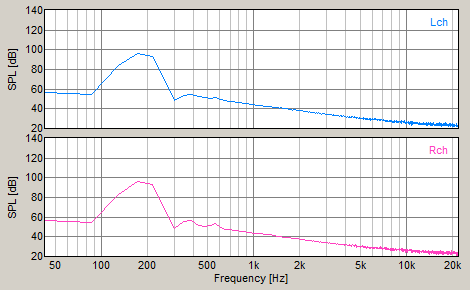
\includegraphics[width=0.45\linewidth]{result/day_4/fft_sine0p5}
		\end{figure}
	\end{exampleblock}
	\end{frame}

	\begin{frame}[fragile]
	\frametitle{Test modifikasi panjang array}
	\begin{exampleblock}{Skala Frekuensi 0.25 atau panjang array 2048}
		Aktual $freq = 86 Hz$ dan $SPL = 92 dB$
		\begin{figure}[H]
			\centering
			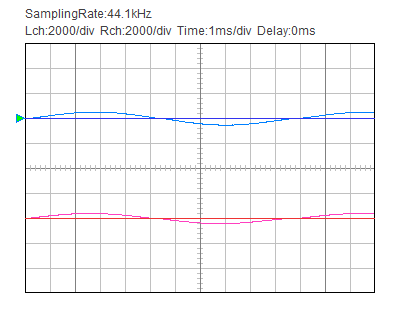
\includegraphics[width=0.4\linewidth]{result/day_4/osi_sine0p25}
			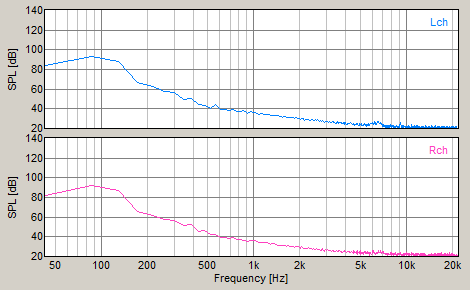
\includegraphics[width=0.45\linewidth]{result/day_4/fft_sine0p25}
		\end{figure}
	\end{exampleblock}
	\end{frame}

	\begin{frame}[fragile]
	\frametitle{Test modifikasi panjang array}
	\begin{exampleblock}{Rangkuman Respon}
		\begin{figure}[H]
			\centering
			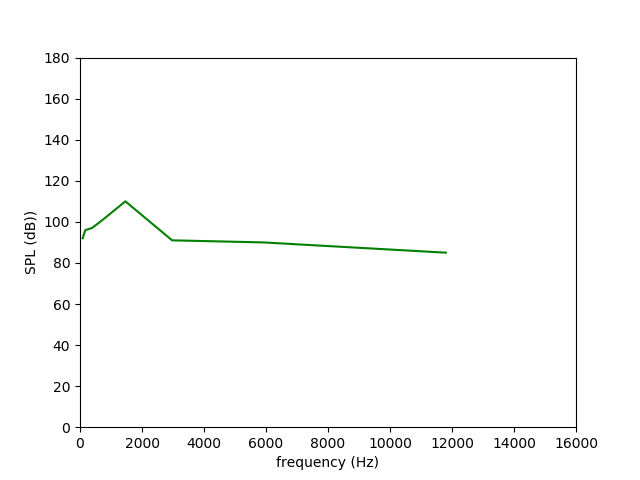
\includegraphics[width=0.45\linewidth]{result/analisa/freq_spl}
			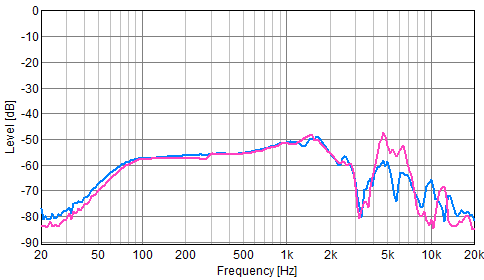
\includegraphics[width=0.45\linewidth]{result/day_1/FreqResp_JBL}
		\end{figure}
	\end{exampleblock}
	\end{frame}

	\begin{frame}[fragile]
	\frametitle{Test modifikasi amplitudo}
	\begin{exampleblock}{}
		Untuk mendapatkan frekuensi 500Hz digunakan panjang array 410.
		\[
		Y(i) =
		\begin{cases}
		S_A C_A sin(2 \pi \frac{i}{410}), \text{ if } Y \geq 0, \text{ for } 0 \leq i < 410\\
		S_A C_A sin(2 \pi \frac{i}{410})+65535, \text{ if } Y < 0, \text{ for } 0 \leq i < 410
		\end{cases}
		\]
		dengan $S_A$ adalah skala 1 sampai 0.0001, dan $C_A=3277$ adalah konstanta amplitudo maksimal
		untuk signed 16-bit yang telah di atenuasi $0.1$.
	\end{exampleblock}
	\begin{exampleblock}{}
		\begin{minted}[frame=lines,fontsize=\footnotesize]{c}
double ampl;
buffsize = (uint16_t) 512/1.25;
for(i=0;i<buffsize;i++){
	ysin = ampl*0.1*32767*sin(2*3.141592653589793*(i/buffsize));
	if(ysin >= 0){ i2s_tx_buf[i]=ysin; }
	if(ysin <0  ){ i2s_tx_buf[i]=ysin+65535; }
}
i2scfg.size = buffsize;
		\end{minted}
	\end{exampleblock}
	\end{frame}

	\begin{frame}[fragile]
	\frametitle{Test modifikasi amplitude}
	\begin{exampleblock}{Skala amplitudo 1}
		Aktual $SPL = 98 dB$
		\begin{figure}[H]
			\centering
			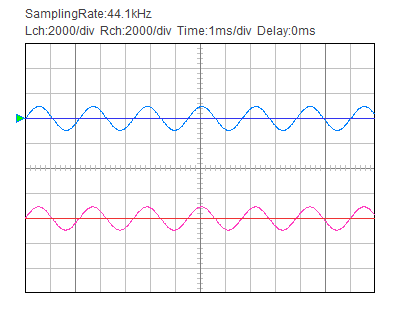
\includegraphics[width=0.4\linewidth]{result/day_4/500Hz/tone1}
			\includegraphics[width=0.45\linewidth]{result/day_4/500Hz/fft_tone1}
		\end{figure}
	\end{exampleblock}
	\end{frame}

	\begin{frame}[fragile]
	\frametitle{Test modifikasi amplitude}
	\begin{exampleblock}{Skala amplitudo 0.5}
		Aktual $SPL = 92 dB$
		\begin{figure}[H]
			\centering
			\includegraphics[width=0.4\linewidth]{result/day_4/500Hz/tone05}
			\includegraphics[width=0.45\linewidth]{result/day_4/500Hz/fft_tone05}
		\end{figure}
	\end{exampleblock}
	\end{frame}

	\begin{frame}[fragile]
	\frametitle{Test modifikasi amplitude}
	\begin{exampleblock}{Skala amplitudo 0.1}
		Aktual $SPL = 72 dB$
		\begin{figure}[H]
			\centering
			\includegraphics[width=0.4\linewidth]{result/day_4/500Hz/tone01}
			\includegraphics[width=0.45\linewidth]{result/day_4/500Hz/fft_tone01}
		\end{figure}
	\end{exampleblock}
	\end{frame}

	\begin{frame}[fragile]
	\frametitle{Test modifikasi amplitude}
	\begin{exampleblock}{Skala amplitudo 0.05}
		Aktual $SPL = 72 dB$
		\begin{figure}[H]
			\centering
			\includegraphics[width=0.4\linewidth]{result/day_4/500Hz/tone005}
			\includegraphics[width=0.45\linewidth]{result/day_4/500Hz/fft_tone005}
		\end{figure}
	\end{exampleblock}
	\end{frame}

	\begin{frame}[fragile]
	\frametitle{Test modifikasi amplitude}
	\begin{exampleblock}{Skala amplitudo 0.01}
		Aktual $SPL = 58 dB$
		\begin{figure}[H]
			\centering
			\includegraphics[width=0.4\linewidth]{result/day_4/500Hz/tone001}
			\includegraphics[width=0.45\linewidth]{result/day_4/500Hz/fft_tone001}
		\end{figure}
	\end{exampleblock}
	\end{frame}

	\begin{frame}[fragile]
	\frametitle{Test modifikasi amplitude}
	\begin{exampleblock}{Skala amplitudo 0.005}
		Aktual $SPL = 51 dB$
		\begin{figure}[H]
			\centering
			\includegraphics[width=0.4\linewidth]{result/day_4/500Hz/tone0005}
			\includegraphics[width=0.45\linewidth]{result/day_4/500Hz/fft_tone0005}
		\end{figure}
	\end{exampleblock}
	\end{frame}

	\begin{frame}[fragile]
	\frametitle{Test modifikasi amplitude}
	\begin{exampleblock}{Skala amplitudo 0.001}
		Aktual $SPL = 42 dB$
		\begin{figure}[H]
			\centering
			\includegraphics[width=0.4\linewidth]{result/day_4/500Hz/tone0001}
			\includegraphics[width=0.45\linewidth]{result/day_4/500Hz/fft_tone0001}
		\end{figure}
	\end{exampleblock}
	\end{frame}

	\begin{frame}[fragile]
	\frametitle{Test modifikasi amplitude}
	\begin{exampleblock}{Skala amplitudo 0.0005}
		Aktual $SPL = 47 dB$
		\begin{figure}[H]
			\centering
			\includegraphics[width=0.4\linewidth]{result/day_4/500Hz/tone00005}
			\includegraphics[width=0.45\linewidth]{result/day_4/500Hz/fft_tone00005}
		\end{figure}
	\end{exampleblock}
	\end{frame}

	\begin{frame}[fragile]
	\frametitle{Test modifikasi amplitude}
	\begin{exampleblock}{Skala amplitudo 0.0001}
		Aktual $SPL = 42 dB$
		\begin{figure}[H]
			\centering
			\includegraphics[width=0.4\linewidth]{result/day_4/500Hz/tone00001}
			\includegraphics[width=0.45\linewidth]{result/day_4/500Hz/fft_tone00001}
		\end{figure}
	\end{exampleblock}
	\end{frame}

	\begin{frame}[fragile]
	\frametitle{Test modifikasi amplitude}
	\begin{exampleblock}{Skala amplitudo 0.0001}
		Aktual $SPL = 42 dB$
		\begin{figure}[H]
			\centering
			\includegraphics[width=0.4\linewidth]{result/day_4/500Hz/tone00001}
			\includegraphics[width=0.45\linewidth]{result/day_4/500Hz/fft_tone00001}
		\end{figure}
	\end{exampleblock}
	\end{frame}

	\begin{frame}[fragile]
	\frametitle{Test modifikasi amplitude}
	\begin{exampleblock}{Rangkuman Respon}
		\begin{figure}[H]
			\centering
			\includegraphics[width=0.45\linewidth]{result/analisa/ampl_scaling}
		\end{figure}
	\end{exampleblock}
	\end{frame}

	\begin{frame}[fragile]
	\frametitle{Terselesaikan}
	\begin{exampleblock}{Model array sinus}
		\[ B = 512/F \]
		\[
		Y(i) =
		\begin{cases}
		A sin(2 \pi \frac{i}{B}), \text{ if } Y \geq 0, \text{ for } 0 \leq i < B\\
		A sin(2 \pi \frac{i}{B})+65535, \text{ if } Y < 0, \text{ for } 0 \leq i < B
		\end{cases}
		\]
		dengan A adalah nilai maksimal variabel \textit{signed 16-bit} yaitu 32767
		dan F adalah skala untuk memodifikasi panjang array buffer.
		Array-Loop pada clock I2S 96MHz dan Sampling BCLK adalah 16kHz.
	\end{exampleblock}
	\begin{exampleblock}{}
		\begin{minted}[frame=lines,fontsize=\footnotesize]{c}
double ampl;
uint16_t buffsize = (uint16_t) 512/freq;
for(i=0;i<buffsize;i++){
	ysin = 0.1*32767*ampl*sin(2*3.141592653589793*(i/buffsize));
	if(ysin >= 0){ i2s_tx_buf[i]=ysin; }
	if(ysin <0  ){ i2s_tx_buf[i]=ysin+65535; }
}
i2scfg.size = buffsize;
		\end{minted}
	\end{exampleblock}
	\end{frame}

	\begin{frame}[fragile]
	\frametitle{Belum Terselesaikan}
	\begin{exampleblock}{}
		\begin{itemize}
			\item Kompensasi headphone yang memiliki respon amplitudo yang
			tidak flat (datar/konstan) terhadap frekuensi.
			
			\item Perbedaan signifikan antara array untuk PCM mono dan array PCM stereo.
			
			\item Masalah \textit{Audio-Pop} yang masih muncul di akhir \textit{tone play}.
		\end{itemize}
	\end{exampleblock}
	\begin{exampleblock}{}
		Pengembangan selanjutnya membutuhkan instrumen \textit{Audio Capture/Analyzer}
		walaupun tidak mengharuskan menggunakan manekin KEMAR (untuk sementara).
	\end{exampleblock}
	\end{frame}

	\begin{frame}
	\frametitle{Achievement}
	\begin{exampleblock}{What is really achievement?}
		\textit{Most basic} dari desain standar untuk tone/audio generator dengan \textit{least noise}.
	\end{exampleblock}
	\begin{exampleblock}{What is "standard" here?}
		Protokol I2S (\textit{Inter-Integrated Sound}) sebagai standar komunikasi data/sinyal audio
		dari microcontroller dan Audio DAC (Digital to Analog Converter). 
	\end{exampleblock}
	\end{frame}

	\begin{frame}
	\frametitle{Care to join?}
	\begin{exampleblock}{Qualification?}
		\begin{itemize}
			\item Suka memperhatikan sesuatu dengan detil.
			\item Menikmati \textit{development-process}.
			\item Mau belajar DSP (\textit{Digital Signal Processing}).
			\item Mau belajar bahasa pemrograman C.
			\item Mau belajar managemen \textit{source-code} Git.
			\item Buka akun Github (gratis) dan daftar membership grup Vibrastic Lab di Github.
		\end{itemize}
	\end{exampleblock}
\end{frame}
	
\end{document}
